\begin{center}
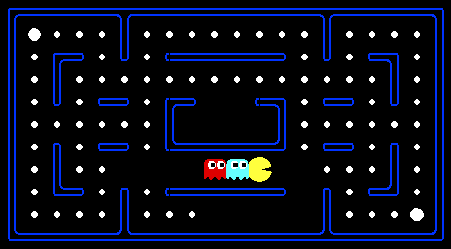
\includegraphics[width=0.5\textwidth]{pacman_multi_agent.png}
\end{center}

{\bf Introduction}

For those of you not familiar with Pac-Man, it's a game where Pac-Man (the
yellow circle with a mouth in the above figure) moves around in a maze and tries
to eat as many {\em food pellets} (the small white dots) as possible, while
avoiding the ghosts (the other two agents with eyes in the above figure). If
Pac-Man eats all the food in a maze, it wins. The big white dots at the top-left
and bottom-right corner are {\em capsules}, which give Pac-Man power to eat
ghosts in a limited time window, but you won't be worrying about them for the
required part of the assignment. You can get familiar with the setting by
playing a few games of classic Pac-Man (instructions provided later).

In this assignment, you will design agents for the classic version of Pac-Man,
including ghosts. Along the way, you will implement both minimax and expectimax
search.

The base code for this assignment contains a lot of files, which are listed
towards the end of this page; you, however, {\bf do not} need to go through
these files to complete the assignment. These are present only to guide the more
adventurous amongst you to the heart of Pac-Man. As in previous assignments, you
will only be modifying |submission.py|.

A basic |grader.py| has been included, but it only checks for
timing issues, not functionality. You can check that Pac-Man behaves as
described in the problems, and run |grader.py| without timeout to test your
implementation. However, the best way to ensure that your implementation does
not time out is to submit test submissions early to Gradescope.
\clearpage

{\bf Warmup}

First, play a game of classic Pac-Man to get a feel for the assignment:

\begin{lstlisting}
(XCS221)$ python pacman.py
\end{lstlisting}

You can always add |--frameTime 1| to the command line to run in "demo mode"
where the game pauses after every frame.

Now, run the provided |ReflexAgent| in |submission.py|:

\begin{lstlisting}
(XCS221)$ python pacman.py -p ReflexAgent
\end{lstlisting}

Note that it plays quite poorly even on simple layouts:

\begin{lstlisting}
(XCS221)$ python pacman.py -p ReflexAgent -l testClassic
\end{lstlisting}

You can also try out the reflex agent on the default |mediumClassic| layout with
one ghost or two.

\begin{lstlisting}
(XCS221)$ python pacman.py -p ReflexAgent -k 1
(XCS221)$ python pacman.py -p ReflexAgent -k 2
\end{lstlisting}

{\em Note: You can never have more ghosts than the layout permits (see
|src/layouts/mediumClassic.lay|).}

{\em Options: Default ghosts are random; you can also play for fun with slightly
smarter directional ghosts using |-g DirectionalGhost|. You can also play
multiple games in a row with |-n|. Turn off graphics with |-q| to run lots of
games quickly.}

Now that you are familiar enough with the interface, inspect the |ReflexAgent|
code carefully (in |submission.py|) and make sure you understand what it's
doing. The reflex agent code provides some helpful examples of methods that
query the |GameState|: A |GameState| object specifies the full game state,
including the food, capsules, agent configurations, and score changes: see
|submission.py| for further information and helper methods, which you will be
using in the actual coding part. We are giving an exhaustive and very detailed
description below, for the sake of completeness and to save you from digging
deeper into the starter code. The actual coding part is very small -- so please
be patient if you think there is too much writing.

{\em Note: If you wish to run the game in the terminal using a text-based
interface, check out the |terminal| directory.}

\clearpage

{\bf Coding Files}

|submission.py|: Where all of your multi-agent search agents will reside, and
the only file that you need to concern yourself with for this assignment.

|pacman.py|: The main file that runs Pac-Man games. This file also describes a
Pac-Man |GameState| type, which you will use extensively in this assignment.

|game.py|: The logic behind how the Pac-Man world works. This file describes
several supporting types like |AgentState|, |Agent|, |Direction|, and |Grid|.

|util.py|: Useful data structures for implementing search algorithms.

|graphicsDisplay.py|: Graphics for Pac-Man.

|graphicsUtils.py|: Support for Pac-Man graphics.

|textDisplay.py|: ASCII graphics for Pac-Man.

|ghostAgents.py|: Agents to control ghosts.

|keyboardAgents.py|: Keyboard interfaces to control Pac-Man.

|layout.py|: Code for reading layout files and storing their contents.

|search.py|, |searchAgents.py|, |multiAgentsSolution.py|: These files are not
relevant to this assignment and you do not need to modify them.

\clearpage
